
\chapter{Online {\IterComp}}

\section{Work-based Performance Metric}\label{sec:metric}

In this section we define the work-based performance (WP) metric proposed for comparing different optimised versions of a program when executing with different inputs.
We define the performance metric as the ratio between the amount of \textit{work}, $\Delta W$, performed during a period of time, $\Delta t$.
\[
   P = \frac{\Delta W}{\Delta t}
\]

%The hypothesis is that, given two optimisations $o_1$ and $o_2$, a program compiled with optimisation $o_2$ would \textit{consistently} perform better than when it is compiled with $o_1$, i.e., $o_1 \tilde{<}_p \, o_2$, if it performs more \textit{work} per unit of time when compiled with $o_2$ instead of $o_1$. 
By measuring the amount of \textit{work} done per unit of time we reduce the impact of input-dependent aspects and focus instead on the efficiency of the optimised program.
For this metric, the main challenge is to precisely define what represents \textit{work}.

%For that purpose, we intend to use profiling techniques to measure the input size and amount of computation performed on the execution path triggered by the input~\cite{ball94,ball96,zaparanuks12,coppa14}.

%In addition to being useful for speeding up {\itercomp} across a large number of different inputs, this metric based on comparing work-based efficiencies could
%potentially be used for applying {\itercomp} \textit{online}.
%However, the overhead for estimating the amount of \textit{work} must be low enough for the performance gains to be beneficial.

We model the computational work $\Delta W$ as a linear equation based on block frequency information and a cost model of the instruction set.
\[
\Delta W = \varepsilon + \sum_{B} w(B)f(B)
\]
where $f(B)$ represents the frequency of basic block $B$ and $w(B)$ represents the computational work of executing $B$.
We define the work of a basic block $B$ as the sum of the cost of its instructions, i.e.,
\[
w(B) = \sum_{i} w_i N_B(i)
\]
where $w_i$ is the cost of instruction $i$ and $N_B(i)$ is the number of occurrences of instruction $i$ in basic block $B$.

In this simplified model, we consider that $w_i$ is constant across all programs and executions in the given target platform.
However, $N_B(i)$ is program dependent but constant across executions, while $f(B)$ is both program and execution dependent, since $f(B)$ can change when executing with different inputs.
In other words, $N_B(i)$ is a static value known at compile-time and $f(B)$ is a dynamic value known only at run-time.
%If we define $x_i$ as
%\[
%x_i = \sum_{B\in P} N_B(i)f(B)
%\]
%we can write our definition of work $\Delta W$ as the following linear equation
%\[
%\Delta W = \varepsilon + \sum_{i\in I} w_i x_i
%\]

%\subsection{Linear regression}
%
%\begin{figure}[htb]
%    \centering
%    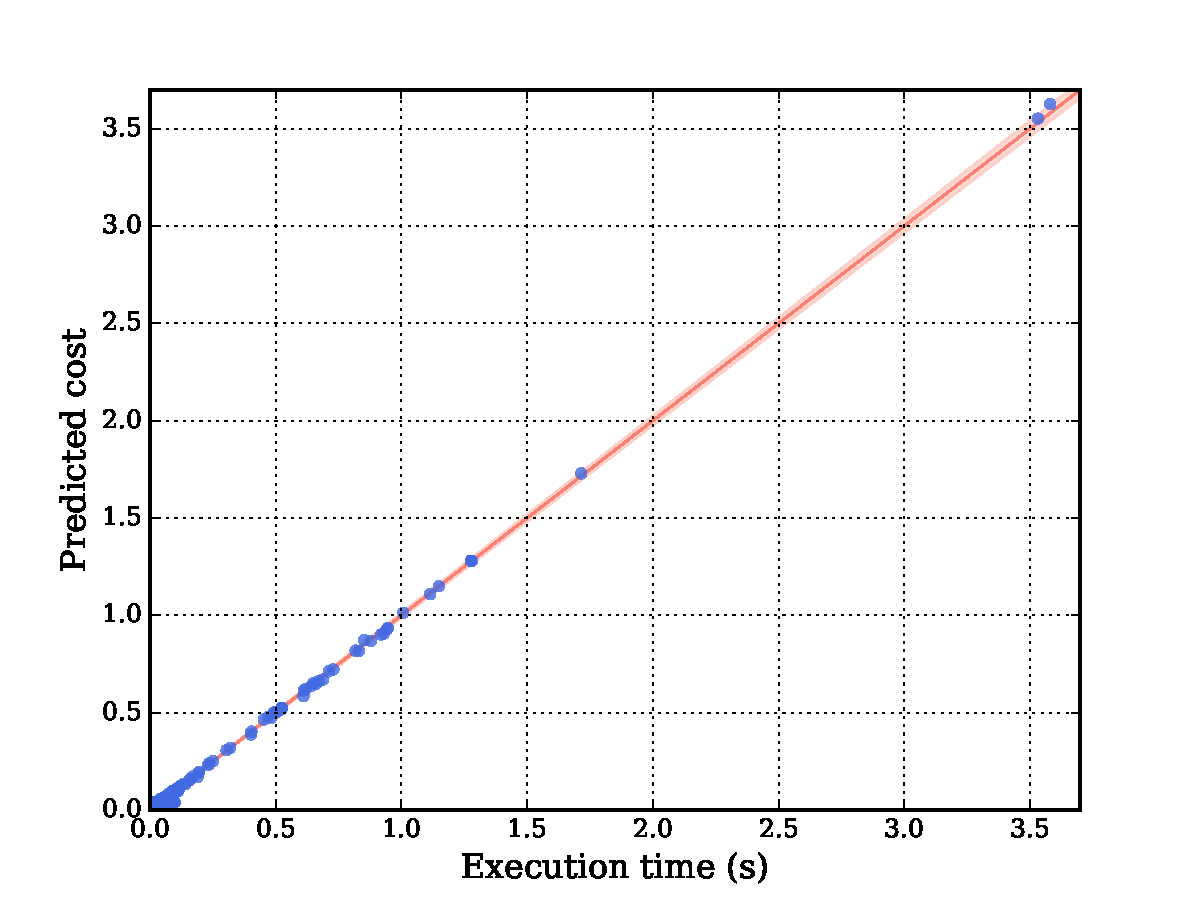
\includegraphics[width=\linewidth]{figs/cost-model.pdf}
%    \caption{Comparison between the naive and optimal instrumentation with no compiler optimisation.} %, i.e., compiled with \textbf{\texttt{-O0}}.}
%    \label{fig:cost-model}
%\end{figure}
%mse 0.000145373168444
%mae 0.00737261168981
%mae* 0.0033892281406
%mape 75.2924320971
%corr (0.99946441743545622, 0.0)

\subsection{Estimating a Cost Model of the Instructions}

Similarly to previous work~\citep{giusto01,powell09,brandolese11}, we derive the cost model of the instruction set by modelling the problem as a multi-variable linear regression, where the \textit{regression coefficients} are the costs of the instructions and the \textit{regressors} are computed as $\sum_B N_B(i)f(B)$ for each instruction $i$.
\[
\Delta W = \varepsilon + \sum_{i} \left(w_i \sum_{B} N_B(i)f(B)\right)
\]

By having some empirical data after executing several benchmarks with different inputs, we can fit the linear model with this empirical data in order to obtain the costs of the instructions.
In order to fit the linear model, we measure the wall-clock time when executing the training benchmarks described in Section\ref{sec:benchmarks} with their respective 1000 input datasets.
For these measurements, the training benchmarks are compiled without optimisation.
The reason for using no optimisation is because it allows to use the trained cost model for computing a work metric which is independent of optimisations, as we explained in Section~\ref{}.

\begin{figure}[htb]
    \centering
    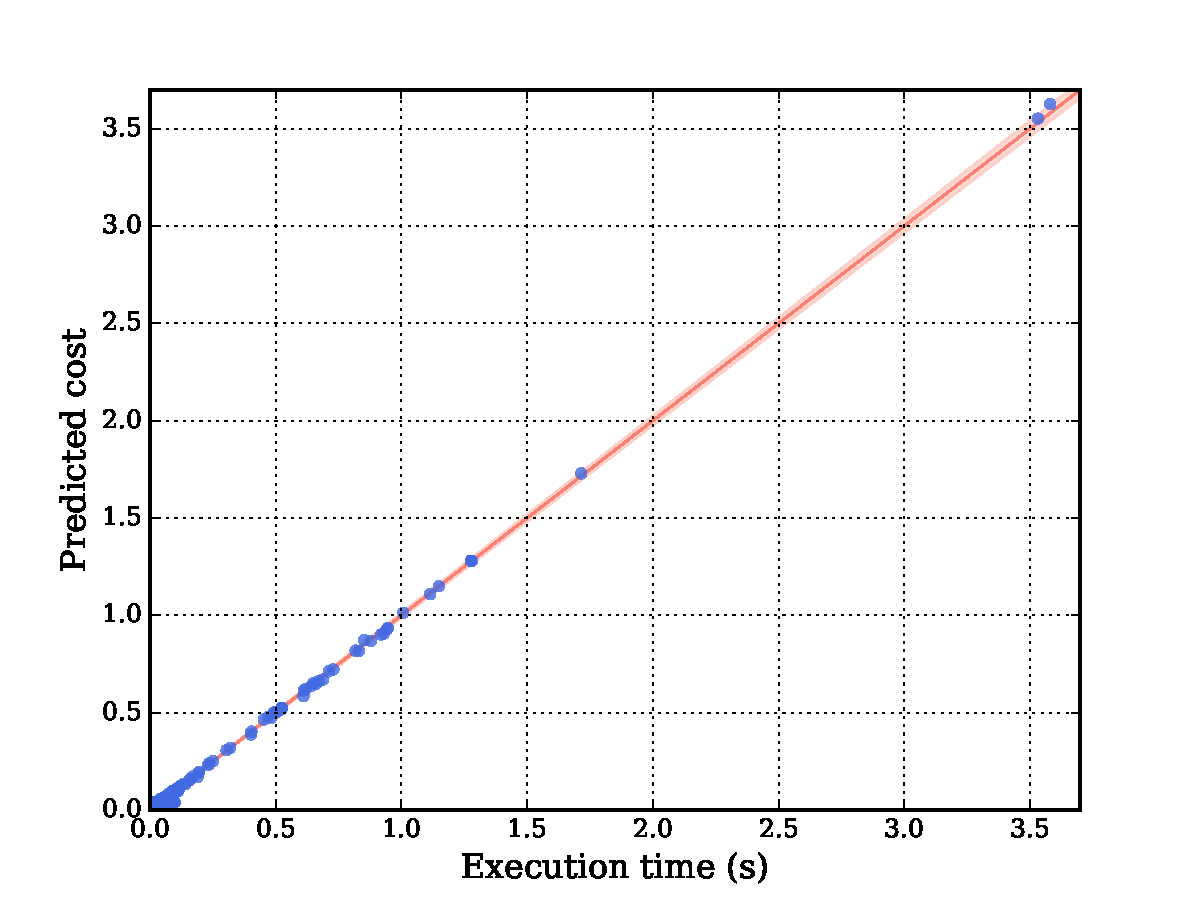
\includegraphics[width=0.9\linewidth]{figs/cost-model.pdf}
    \caption{Linear model fitted from empirical data. The mean absolute error (MAE) for the fitted curve is of 7 milliseconds.}
    \label{fig:cost-model}
\end{figure}

Because we fit the linear model based on the wall-clock execution time, the derived cost model can be interpreted as an estimate of the execution time when the program is compiled without optimisations.
Figure~\ref{fig:cost-model} compare the work metric with the corresponding execution time for some instances of the test benchmarks.
Notice how the fitted model has a higher relative error for the instances with very short execution time, namely those that run for less than one tenth of a second.
The mean absolute error (MAE) for the fitted curve is of 7 milliseconds.

\subsection{Comparison with Instructions Per Cycle} \label{sec:ipc-vs-work-metric}

The IPC metric have been widely used for studying performance benefits of hardware optimisations.

The proposed WP metric differs from IPC in a key aspect:
the IPC metric is computed soley on the final optimised program.
For different optimisations of the same program, both the number of instructions and the number of cycles can change for the same input.
On the other hand, WP computes the amount of work based on the unoptimised program, which means that it always consider the same amount of work for the same input, regardless of the optimisations applied on the program.

For this reason, higher IPC does not necessarily translates to shorter execution time.
We can illustrate this fact with an example as shown in Table~\ref{}.
Although program P1 has twice the IPC of P2, P1 is one cycle slower than P2.
As this example illustrates, the IPC metric can be misleading when compared different versions of the same program.

\begin{table}[h]
\centering
\begin{tabular}{|c|c|c|c|}
\hline
                       & P1 & P2  \\
\hline
Number of Instructions & 5  & 2   \\
Number of Cycles       & 5  & 4   \\
IPC                    & 1  & 0.5 \\
\hline
\end{tabular}
\caption{Example that illustrates that a higher IPC does not necessarily translates to shorter execution time.}
\label{tab:ipc-example}
\end{table}

\section{Online {\IterComp} Infrastructure} \label{sec:oic-infra}

Although {\itercomp} had been originally proposed as an \textit{offline} optimisation strategy it can also be adapted to work in the online scenario.
Instead of selecting the best optimisation sequence as part of the development time (pre-shiping) of a program, a first version of the program is shipped together with a {\itercomp} mechanism.
In the online scenario, the program is shipped with a initial optimisation sequence and different optimisation sequences are evaluated as the end-user executes the program.
This optimisation strategy is also known as idle-time optimisation, as the re-compilation happens between runs of the program.

LLVM is particularly suitable for iterative compilation as it makes possible to cache a pre-compiled, but still unoptimised, version of the input program in the bitcode format of the LLVM IR.  
This caching allows to speedup the time required for re-compilation as it is able to bypass the frontend phase.
If re-compilation time is critical, it would also be possible to keep only the hot portion of the code in the LLVM bitcode format, while the remaining portion of the code is already in the format of object code.
However, this is out of the scope of this work and we always re-compile the whole program.

\begin{figure}[htb]
    \centering
    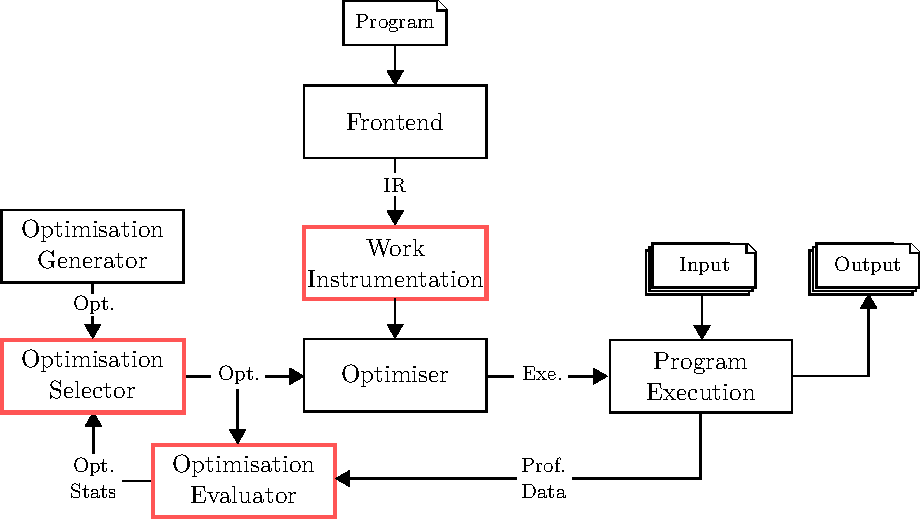
\includegraphics[width=\linewidth]{figs/infra-diagram}
    \caption{Overview of the execution engine for applying {\itercomp}.}
    \label{fig:infra-diagram}
\end{figure}
%\textbf{Describe the process step by step.}

Figure~\ref{fig:infra-diagram} shows an overview of the infrastructure required for applying online {\itercomp},
using WP as the metric of choice for evaluating optimisation sequences.
The online {\itercomp} follows as described bellow:
\begin{enumerate}
\item The program is pre-compiled to the LLVM bitcode format without optimisation.
\item The unoptimised program is instrumented for work profiling.
\item Execution-based optimisation seach:
 \begin{enumerate}
   \item The current optimisation sequence is used for the re-compilation of the program.
   \item The program is executed with any input provided by the end-user.
         During the execution of the program, wall-clock time and the work metric are recorded by profiling instrumentation.
   \item If the recorded profiling for the current optimisation can be used to compute an average performance measurement within a small confidence interval,
         then a new optimisation sequence is generated.
         Otherwise, the same optimisation sequence is used for the next execution.
 \end{enumerate}
\end{enumerate}

In this work we focus mainly on the highlighted components.
The \textit{Work Instrumentation} phase focuses on providing a low-overhead instrumentation for profiling the work metric.
The instrumentation consists in adding a global counter to the program which is used to accumulate the amount of work computed during the program's execution, by means of the cost model of the instruction set.
A detailed description of the work instrumentation is presented in Section~\ref{chap:instr}.

%In both phases the goal is to improve the performance of the execution phase, but from different perspectives.
%\textit{(i.)} In the compilation phase we focused on providing a low-overhead instrumentation for profiling the work metric. This phase is responsible to improve performance by lowering the overhead of the work profiling.
%\textit{(ii.)} In the evaluation phase we proposed the use of the WP metric in order to enable {\itercomp} in an online scenario.
%This phase is responsible to improve performance by being able to properly assess different optimisations such that the best optimisation can be selected.
%Chapter~\ref{chap:instr} describes our work profiling strategy and Section~\ref{sec:metric} describes the work-based metric.

%\textbf{Talk about the process of keeping the same optimization for a given input-window and how the optimizations as selected based on the evaluation of these "evidences". Perhaps we could suggest using the Theory of Evidences at this point?!}

In most online scenarios, it is common for periods of peak usage and idle periods.
For example, mobile devices are usually intensely used during the day, with some idle periods at night while its battery is being re-charged.
The proposed infrastructure is very well suited for these online scenarios as multiple runs of the program can be monitored during peak time, by collecting the work profiling and measuring its execution time, while at the idle time, the profiling statistics can be used for selecting better optimisations and re-compiling the program.
However, if idle time is almost non-existent, the proposed infrastructure can still be used by re-compiling the program with a different optimisation while multiple runs of the program are being executed.

